%------------------------------------------------------------------------------
%   PACKAGES AND OTHER DOCUMENT CONFIGURATIONS
%------------------------------------------------------------------------------

\documentclass[twoside,twocolumn]{article}

%\usepackage[sc]{mathpazo} % Use the Palatino font
%\usepackage[T1]{fontenc} % Use 8-bit encoding that has 256 glyphs
%\linespread{1.05} % Line spacing - Palatino needs more space between lines
%\usepackage{microtype} % Slightly tweak font spacing for aesthetics

\usepackage[english]{babel} % Language hyphenation and typographical rules

% Document margins
\usepackage[hmarginratio=1:1,top=32mm,left=20mm,right=20mm,columnsep=20pt]{geometry}
% Custom captions under/above floats in tables or figures
\usepackage[hang, small,labelfont=bf,up,textfont=it,up]{caption}
\usepackage{booktabs} % Horizontal rules in tables

\usepackage{enumitem} % Customized lists
\setlist[itemize]{noitemsep} % Make itemize lists more compact
\usepackage{textcomp}

% Allows abstract customization
\usepackage{abstract}
% Set the "Abstract" text to bold
\renewcommand{\abstractnamefont}{\normalfont\bfseries}
% Set the abstract itself to small italic text
\renewcommand{\abstracttextfont}{\normalfont\small\itshape}

\usepackage{fancyhdr} % Headers and footers
\pagestyle{fancy} % All pages have headers and footers
\fancyhead{} % Blank out the default header
\fancyfoot{} % Blank out the default footer
\fancyhead[C]{\thetitle}
\fancyfoot[RO,LE]{\thepage} % Custom footer text

\usepackage{titling} % Customizing the title section

\usepackage{hyperref} % For hyperlinks in the PDF
\usepackage{amsmath}

\usepackage{tikz}
\usetikzlibrary{bayesnet}
\usetikzlibrary{arrows}

\usepackage{color}
\usepackage{caption}
\usepackage{subcaption}

\usepackage{graphicx}

\captionsetup[figure]{labelfont={bf},textfont=normalfont}

%------------------------------------------------------------------------------
%   TITLE SECTION
%------------------------------------------------------------------------------

\setlength{\droptitle}{-4\baselineskip} % Move the title up

\pretitle{\begin{center}\Huge\bfseries} % Article title formatting
\posttitle{\end{center}} % Article title closing formatting

\title{MT Project Proposal: \\ Using Neural Networks to Learn Word Alignments}
\author{%
\textsc{Bailey Parker} \\[1ex]
\normalsize Johns Hopkins University \\
\normalsize \href{mailto:bailey@jhu.edu}{bailey@jhu.edu}
 \and
 \textsc{Vivian Tsai} \\[1ex]
\normalsize Johns Hopkins University \\
\normalsize \href{mailto:viv@jhu.edu}{viv@jhu.edu}
 \and
  \textsc{William Watson} \\[1ex]
\normalsize Johns Hopkins University \\
\normalsize \href{mailto:wwatso13@jhu.edu}{wwatso13@jhu.edu}
}

\date{}%\today} % Leave empty to omit a date
% \renewcommand{\maketitlehookd}{%

% }

%------------------------------------------------------------------------------
\DeclareMathOperator*{\argmax}{arg\,max}
\newcommand{\qdist}[1]{\ifmmode\langle#1\rangle\else\textlangle#1\textrangle\fi}


\begin{document}

% Print the title
\maketitle

%------------------------------------------------------------------------------
%   ARTICLE CONTENTS
%------------------------------------------------------------------------------

% \section{Introduction}

% TODO

%------------------------------------------------

\begin{abstract}
% \noindent \blindtext
We seek to explore the word alignment problem with the help of neural networks. More specifically, we want to see if the original Expectation-Maximization (EM) approach to word alignment can be transcribed as a neural network in a supervised and unsupervised setting.
\end{abstract}

% REMEMBER IDEA IS TOO COPY PROPOSAL INTO FINAL WRITEUP

\section{Introduction}
% WHAT IS OUR METRIC!!!
Word Alignment seeks to match individual words in a parallel corpus such that the Alignment Error Rate (AER) is minimized. In a previous assignment, our task was to implement IBM Model 1, based on the Expectation-Maximization (EM) algorithm. Following IBM Model 1, we implemented a reparametrization of IBM Model 2 that favors alignments along the diagonal. Finally, we implemented an Alignment by Agreement Model that trained a French to English and English to French model and combined the results to make better alignments.

Our proposal for this project is to replace the EM algorithm and reparametrization of IBM Model 2 with a neural network architecture. In addition, the model will incorporate Alignment by Agreement. We will use PyTorch to build the model and loss functions. The key concept is that we can create a loss function that the network will learn the optimal parameters to learn word alignments from a corpus of parallel text.


\section{Background}
Our approach is inspired by current research in topic modeling with Latent Dirichlet Allocation (LDA) models. LDA models are generative probabilistic models that model topics across distributions of words in a corpus. LDAs are based on variational methods and EM for Bayes parameter estimation.

% exoand this section, and say that the work is inspiration to our approach
applying a NN to approximate the posterior distributions.\\
see apibm - apply tech to lda.\\
LDA PAPER\footnote{\url{http://www.jmlr.org/papers/volume3/blei03a/blei03a.pdf}}
VAE PAPER\footnote{\url{https://arxiv.org/pdf/1312.6114.pdf}} 

% INSERT GRAPHIC OF PLATE DIAGRAM FOR LDA HERE!
% Also cite LDA paper.
\begin{figure*}
\centering
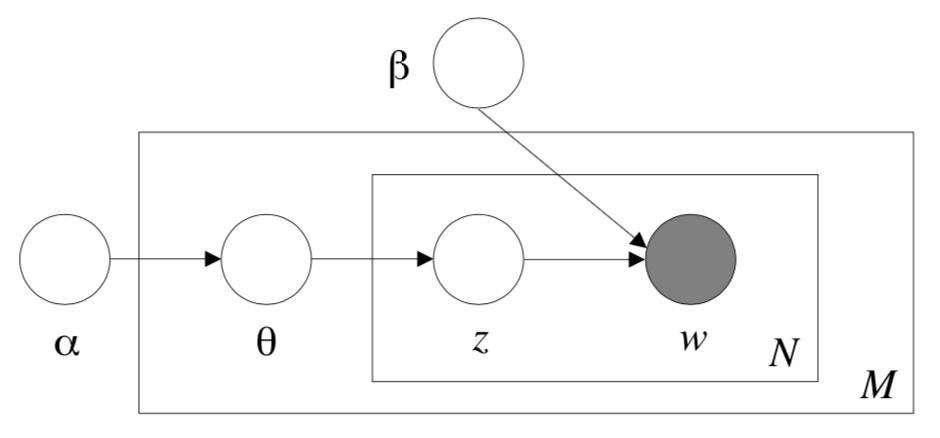
\includegraphics[scale=0.5]{LDADiagram}
\caption{Graphical model representation of LDA. The boxes are “plates” representing replicates. The outer plate represents documents, while the inner plate represents the repeated choice of topics and words within a document. }
\end{figure*}

Current research attempts to supplant the probabilistic modeling with a neural network architecture. 

Additional inspiration comes from Variational Auto-Encoders (VAE).
% Expand discussion on VAE and similiarity to our proposal. MAybe include VAE diagram.

\section{Original Formulation}
% Can steal shorten version from original paper! yay!

IBM Model 1 estimates the translation probabilities of the data through the EM algorithm\footnote{\url{http://mt-class.org/jhu/assets/papers/alopez-model1-tutorial.pdf}}. The EM algorithm is useful in discovering and learning the parameters of a latent variable model. 

Once we are done training the model, to make an alignment guess, we must find the alignment that returns the maximum probability. For some alignment $a_i$:
\begin{equation}
\hat{a}_i = \argmax_{a_i} \, t(e_{a_i}|f_j)
\end{equation}
where $t(e_{a_i}|f_j)$ is the translation probability obtained by IBM Model 1. This will give us the English word $e_{a_i}$ that is the most likely translation of the French word $f_j$.

The work of Dyer et al.\footnote{\url{http://aclweb.org/anthology/N/N13/N13-1073.pdf}} added an effective reparameterization of IBM Model 2 to give an alignment distribution $a$. We define for a French sentence \textbf{f} of length $n = |\textbf{f}|$, an English sentence \textbf{e} of length $m=|\textbf{e}|$, with precision parameter $\lambda$, the alignment distribution $a$ as follows:

\begin{equation}
\begin{split}
h(i,j,m,n) = - \left| \frac{i}{m} - \frac{j}{n}\right| \\
\\
a(i,j,m,n) =e^{  \lambda h(i,j,m,n)} \\
\end{split}
\end{equation}


This formulation gives us a position aware distribution that favors alignments towards the diagonal for a given English word $e_i$ and French word $f_j$. The precision parameter $\lambda$ controls how strongly the model prefers the diagonal.

Finally, incorporating the Alignment by Agreement model improvement was inspired by the work done by Liang et. al.\footnote{\url{http://aclweb.org/anthology/N/N06/N06-1014.pdf}}. However, our original implementation was strongly influenced by the pseudocode used in the \texttt{Grow-Diag-Final} Alignment Heuristic by the Moses Statistical Translation System\footnote{\url{http://www.statmt.org/moses/?n=FactoredTraining.AlignWords}}. 

We trained an EM model in both directions, one for English to French, $A_{E \rightarrow F}$, and another for French to English, $A_{F \rightarrow E}$. Using the alignments generated by each individual model, we then proceed to take the intersection of each model's alignments. 
\begin{equation}
Intersection = A_{E \rightarrow F} \, \bigcap \, A_{F \rightarrow E}
\end{equation}
\begin{equation}
Union = A_{E \rightarrow F} \, \bigcup \, A_{F \rightarrow E}
\end{equation}
This effectively gives us an alignment matrix that both models favor strongly, i.e. agree on. From this intersection matrix, we can then use the \texttt{GROW-DIAG-FINAL} algorithm to fill in the remaining gaps from the union of alignments. 


\section{Our Formulation}
% basically regurtiate (nicely) what was on board. Maybe make fancy diagrams and stuff.
% also embeddings, positional, POS tagging, etc.

Thank you Koehn, very cool!

% alignment distirbution, i is target position, j is source position, lambda and null p_0
\begin{equation}
a(i, j \, | \, \lambda, p_0) =
\begin{cases} 
      p_0 & \text{if } null \\
     (1-p_0) \cdot e^{-\lambda | \frac{i}{m} - \frac{j}{n}|} & \text{else}
   \end{cases}
\end{equation}


\begin{figure}
\centering
\begin{tikzpicture}

  % Define nodes
  \node[obs]                               (t) {$t$};
  \node[latent, above=0.75cm of t] (a) {$a$};
  \node[latent, above=0.75cm of a, xshift=-0.6cm] (lambda) {$\lambda$};
  \node[latent, above=0.75cm of a, xshift=0.6cm]  (null) {$p_0$};
  \node[obs, right=0.75cm of t]            (s) {$s$};
  \node[latent, below=0.95cm of t]            (theta) {$\theta$};

  % Connect the nodes
  \edge {null,lambda} {a} ; %
  \edge {a,s, theta} {t} ; %

  % Plates
  \plate [xscale=1.75, yscale=1.25] {t} {(a)(t)} {$\quad$} ;

\end{tikzpicture}
\caption{Probabilistic Plate Diagram for Word Alignment, where $t$ is target, $s$ is source, $\theta$ is the translation probability, $\lambda$ is a position parameter, $p_0$ is the null probability, and $a$ is the alignment distribution.}
\end{figure}

\section{Data}
% talk about subtitle extraction. Also labeling of data for supervised? Or should that go in supervised trainign section. Get Bailey to metnion Nikita metric for baseline on unaligned corpus.

\section{Training}

\subsection{Supervised Training}
% cut out top half of model, talk about how we will label our data and incoropoate

\subsection{Unsupervised Training}
% 5 term loss function

\section{Expectation}
% Our Hopes and Dreams!


\begin{equation}
\centering
\begin{split}
\textit{le chat} &\mapsto \textit{the cat} \\
\textit{est} &\mapsto \textit{is} \\
\textit{noir} &\mapsto \textit{black} \\
\end{split}
\end{equation}


% papers with footnote url cite
Alignment By Agreement \footnote{\url{http://aclweb.org/anthology/N/N06/N06-1014.pdf}} 

Diagonal Priors \footnote{\url{http://aclweb.org/anthology/N/N13/N13-1073.pdf}} 

ATIVM \footnote{\url{https://arxiv.org/pdf/1703.01488.pdf}} 

VAE \footnote{\url{https://arxiv.org/pdf/1312.6114.pdf}} 

LDA \footnote{\url{http://www.jmlr.org/papers/volume3/blei03a/blei03a.pdf}} 

\end{document}
